\documentclass{article}

% Macros to make this problem look like the rest of our problems.
\usepackage{icpc_problem}

% Title of your problem.
\title{G: Swarms as a Service}

% Who made the problem
\author{Kyle Morris}
\usepackage{graphicx}
\usepackage{needspace}

% Keywords, from a set of standard keywords.
\keywords{problem}

% Anything you want to say about the problem, including how one could solve it
\comments{comment}

% Difficulty on a 1..10 scale.
\difficulty{2}

\begin{document}

% Plain English description of the problem
\begin{problemDescription}
It's the year 2050, and SaaS (Swarms as a Service) has become the norm. SaaS involves large groups of robots (called swarms) that deliver consumer goods throughout the skies. As a stationary observer, you want to ensure that all of the robots flying above you have stable dynamics. You do this by sampling the swarms state at two different times (t1, t2).
When we look at the swarm between any two states, we first want to determine if the swarm has maintained formation, or if it entering unstable dynamics.

A swarm exhibits stable dynamics if the robots forming the outer boundary of the swarm of state 1, are the same robots in the outer boundary of state 2 (i.e, if you took an elastic band and wrapped it around the robots, the outer boundary is formed by all robots touching the elastic band.)
\end{problemDescription}

\begin{center}
\includegraphics[width=0.8\linewidth]{images/graphic_swarm_invalid}
\\
\caption{example 1: Unstable swarm dynamics. Robot #3 has left the outer boundary of the swarm. Furthermore robot #7 becomes part of the outer boundary.}
\label{fig:sp500_long_results_zoomed}
\end{center}

\begin{center}
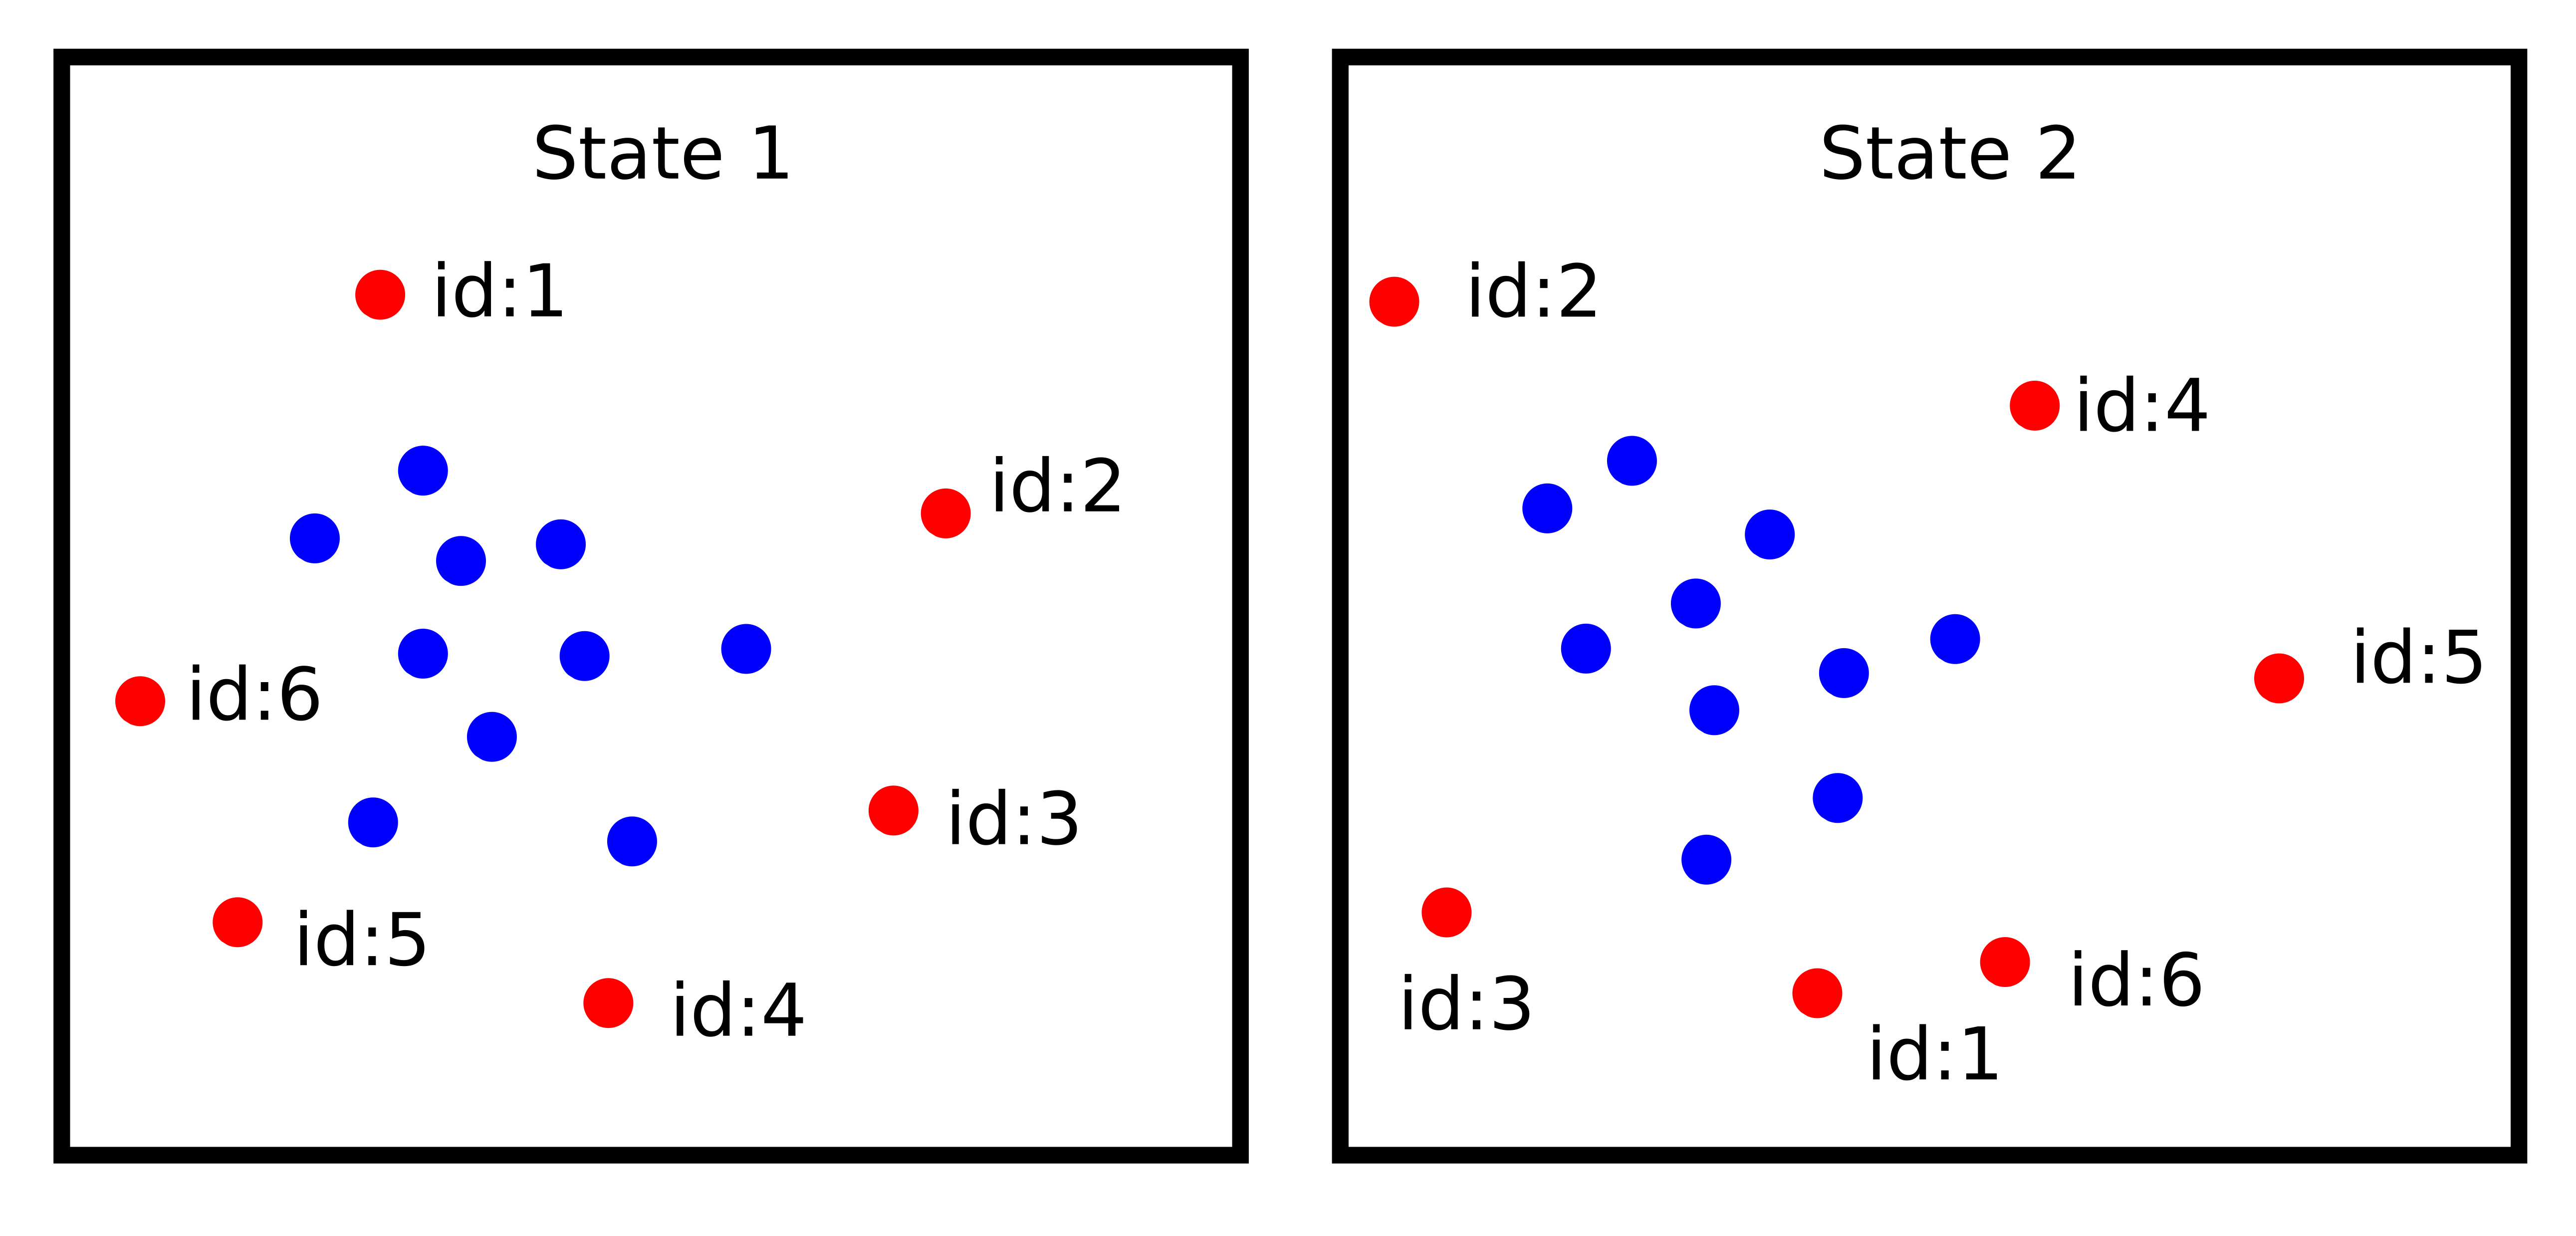
\includegraphics[width=0.8\linewidth]{images/graphic_swarm_valid.png}
\\
\caption{example 2: Stable swarm dynamics. The robots [1,2,3,4,5,6] are surrounding the swarm in both states, despite changing their positions.}
\label{fig:sp500_long_results_zoomed}
\end{center}

\needspace{5em}
\\
% Specific input definition
% Includes what is being taken as input, and in what format
\begin{inputDescription}
Each case will begin with an input containing an integer $N$ being the number of robots in the swarm. $0 \leq N \leq 100$

The following 2N lines contain space separated integers $p_i x_i y_i$, where $p_i$ is the id of the ith robot and $x_i$ and $y_i$ represent the x and y coordinates of the ith robot.
The first N of these values represent the state of the N robots at time $t_1$. The second batch of N lines represents the state of swarm at time $t_2$

Input is complete once you read in a single "0" indicating a swarm with no robots. 
\end{inputDescription}

% Specific output definition
% Includes what should be printed, and in what format
\begin{outputDescription}
Output TRUE If the swarm is stable between states 1 and 2.
Output: FALSE If the swarm is not stable between states 1 and 2. 
\end{outputDescription}

\begin{sampleInput}
4
1 5 2
2 1 3
3 1 5
4 4 4
1 2 4
2 1 3
3 1 5
4 4 4
3
1 2 4
2 1 3
3 1 5
1 333 666
2 420 69
3 391 5
0
\end{sampleInput}
\begin{sampleOutput}
FALSE
TRUE
\end{sampleOutput}

\end{document}
